\section{P2P Wire Protocol}
%TODO:some diagrams to show interactions as well as formally defining p2p node interactions

Nodes on the Centrifuge peer to peer network communicate using the Centrifuge Wire Protocol, which utilizes libp2p\footnote{\url{https://libp2p.io/}} streams as the underlying network transport layer.

\subsection{Usage of libp2p}
libp2p provides building blocks for constructing peer to peer distributed systems and protocols. The Centrifuge network relies on the following components of libp2p for its functionality: 

\subsubsection{Node Identifier (PeerID)} \label{sec:node_id}
A node in a libp2p network must generate a public-private key pair in order to participate in the network. The node's identifier is the multihash\footnote{\url{https://github.com/multiformats/multihash}} or the sha2-256 hash of its public key, and is also known in libp2p terminology as the PeerID\footnote{\url{https://github.com/libp2p/go-libp2p-peer}}. 

\subsubsection{Node Discovery}
Discovery of a node in a libp2p network happens mainly through distributed hash table which works as key-value store to map a node's identifier to its physical location. Centrifuge network uses the Kademlia DHT implementation\footnote{\url{https://github.com/libp2p/go-libp2p-kad-dht}} provided by libp2p. The DHT based discovery works in two stages. The first stage of discovery is the connection to bootstrap nodes which are hard-coded into the node's configuration at the start. Bootstrap nodes allow newly joining or restarting nodes to query the updated DHT and refresh their own list of known peers(peer store) based on that. Centrifuge provides several sets of bootstrap nodes corresponding to different Ethereum networks such as Rinkeby or Kovan. Each set of bootstrap nodes together with the smart contracts which are deployed on the corresponding Ethereum network defines a Centrifuge network. For example, as of the time of writing, the \texttt{RussianHill} Centrifuge network corresponds to bootstrap nodes and smart contracts which are deployed on the Ethereum \texttt{Rinkeby} testnet. 

Once a Centrifuge node is connected to the bootstrap nodes on Centrifuge network, and has updated its peerstore, the second stage of discovery starts. This is through receiving updates to the DHT from the nodes peers using the DHTs P2P protocol. All nodes in the Centrifuge network use the \texttt{centrifuge-dht} content topic to subscribe and publish their availability to other nodes in the network. When there is an update to the content of the topic all nodes in the network receive notifications.

\subsubsection{Encrypted Transport} \label{encrypted transport}
libp2p defines a common network security transport interface. Centrifuge uses the secio\footnote{\url{https://github.com/libp2p/go-libp2p-secio}} implementation of that interface to create encrypted connections between the network nodes. The secio library executes the following steps, similarly to a TLS handshake, to establish a secure, encrypted channel to a remote node. 
\begin{enumerate}
  \item Propose and obtain agreement for supported exchanges, ciphers and hashes together with the public key of the proposer node for identification.
  \item Perform \texttt{Elliptic-curve Diffie-Hellman} key exchange and generate a shared secret key. Here, the node's public key (node identifier) is used for initial message authentication.
  \item Verify encryption using the new shared secret.
\end{enumerate}

Once the shared secret key is established, it is used for encryption of all traffic on the channel. A brief description about libp2p encryption philosophy is available in the encryption spec\footnote{\url{https://github.com/libp2p/specs/blob/master/3-requirements.md\#33-encryption}}.

\subsubsection{Stream Multiplexing}
The ability to multiplex protocols at multiple levels of the networking stack is a defining characteristic of libp2p with multi-multiplexing features\footnote{\url{https://github.com/libp2p/specs/blob/master/3-requirements.md\#32-multi-multiplexing}}. Multiplexed protocol identifiers are strings in the form \texttt{/protocol-name/<optional string1>/../<optional string n>}. For example, \texttt{/http/v2}. A program can register handlers for each of these protocols in the libp2p host and it will take care of routing the messages of a protocol to the appropriate handler. 

Centrifuge uses TCP level stream multiplexing with libp2p to support multiplexing of stream traffic intended for different Centrifuge accounts (\texttt{DID}s) to a single TCP port in a node. Refer section \ref{sec:p2p_multi_account} for more details.

\subsection{Associating a Node(PeerID) with a DID}\label{did-node}

An identity on the Centrifuge network needs to be associated with a node in order for it to be able to perform Centrifuge-specific actions such as creating and signing documents. As introduced in section \ref{sec:node_id}, a node's public key serves as its identity on the Centrifuge network. Therefore, to associate a node to a DID, the DID identity contract (appendix \ref{sec:identity_contract}) on Ethereum stores its associated node's public key(ed25519) with the purpose ID - \texttt{P2P\_DISCOVERY}. From the DID perspective, this key is known as the \texttt{P2P Discovery Key}, as any known Centrifuge DID can be looked up for its associated p2p node id using the method \texttt{getKeyByPurpose} with the purpose ID - \texttt{P2P\_DISCOVERY} (refer section \ref{sec:key_types}). TODO explain that its only one to one association right now


\subsection{Multi-account(DID) handling} \label{sec:p2p_multi_account}

A node in the Centrifuge network can identify traffic associated with a single DID even at the wire protocol level. This is achieved through the use of libp2p stream multiplexing. A protocol identifier on Centrifuge networks is of the form \texttt{/centrifuge/<protocol-version>/<DID>}. Therefore, once a node has received a request and established a connection with a certain protocol identifier, for example \texttt{/centrifuge/v0.0.1/0x5571ecda2005a9B005014817607d02b4E1B7eAff}, it needs to:
\begin{enumerate}
  \item Verify that it can handle version v0.0.1 of the Centrifuge Protocol or reject the request.
  \item Verify that it has been associated to the account with DID \texttt{0x5571ecda2005a9B005014817607d02b4E1B7eAff} to handle or reject the request \ref{did-node}.
  \item Handle the request.
\end{enumerate}
The use of libp2p multiplexing for DID traffic segregation also offers the advantage of using separate ephemeral keys for encryption of DID-specific traffic.

\subsection{Connection and Authentication Layers}

There are two layers of authentication for establishing a connection between two nodes in the Centrifuge network. Following are the steps in the connection establishment flow.

\begin{enumerate}
  \item Given a protocol action, look up relevant node ids to interact with. For example, given a document update, find the node ids of the collaborators using their DIDs (refer \ref{did-node}).
  \item Run the libp2p handshake to establish an authenticated, encrypted channel between the two libp2p nodes (refer \ref{encrypted transport}). This is authentication layer 1.
  \item Now the receiving node needs to authenticate the senders DID (refer \ref{item:sender_auth}). This is the authentication layer 2.
\end{enumerate}

\subsection{Protocol Envelope}\label{sec:protocol_envelope}

All requests and responses exchanged on the Centrifuge network must comply to the Google protobuf based \texttt{protocol envelope} format shown in figure \ref{fig:protocol_envelope}. The \texttt{body} field of the envelope contains the serialized protocol message while the \texttt{header} field includes a set of header fields for the following purposes.

\begin{enumerate}
  \item \texttt{network\_identifier} identifies the Centrifuge network the sender node belongs to. The receiving node would validate its belonging to the same network or else reject the message.
  \item \texttt{node\_version} is the version of the node software that the message originating node is running. Again, the receiving node would reject the message if the received version is incompatible with the version of software that it is running.
  \item \texttt{sender\_id} is the sender's DID (see \ref{did}). Because any DID on the Centrifuge network must be associated with a node on the network using the \texttt{P2P Discovery Key}, the receiving node validates that originating node is, in fact, associated with the sender's DID on Ethereum. Otherwise, it rejects the request. \label{item:sender_auth}
  \item \texttt{type} is included in the message header such that message body bytes could be decoded into the correct type to be processed by the receiving node.
\end{enumerate}

\begin{figure}[h]
  \caption{Protocol envelope}
  \label{fig:protocol_envelope}
  \begin{lstlisting}
  message Envelope {
    Header header = 1;
    bytes body = 2;
  }

  // Header above is defined as
  message Header {
    uint32 network_identifier = 1;
    string node_version = 2;
    bytes sender_id = 3;
    // Body message type
    string type = 4;
  }\end{lstlisting}
\end{figure}



\subsection{Generic P2P Message Envelope}
Wire level message encoding for the Centrifuge protocol is performed by the P2P messenger utility\footnote{\url{https://github.com/centrifuge/go-centrifuge/tree/develop/p2p/messenger}}, hereinafter referred to as the messenger. A generic P2P message envelope shown in figure \ref{fig:generic_envelope}, implemented using Google Protobufs, is used by the messenger to offer a common interface for all Centrifuge p2p network traffic. 

\begin{figure}[h]
  \caption{Generic P2P message envelope}
  \label{fig:generic_envelope}
  \begin{lstlisting}
  message P2PEnvelope {
    bytes body = 2;
  }\end{lstlisting}
\end{figure}

When a protocol envelope based(see \ref{sec:protocol_envelope}) request or a response needs to be sent to a peer node, the initiating node creates an instance of the generic message envelope and sets the serialized bytes of the request or the response in to the body field. Then, the created envelope is passed on to the messenger. The messenger in turn serializes it to the protobuf encoding format\footnote{\url{https://developers.google.com/protocol-buffers/docs/encoding}}, and writes the serialized bytes to the wire using a length delimited format shown in figure \ref{img:generic_message_encoding}. The message length header shown is encoded using varint format\footnote{\url{https://developers.google.com/protocol-buffers/docs/encoding\#varints}}.

\begin{figure}[h]
  \centering
  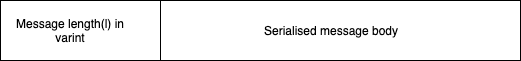
\includegraphics[width=11cm]{img/generic-message-encoding.png}
  \caption{generic message envelope encoding} 
  \label{img:generic_message_encoding}
\end{figure}

Maximum length(\textit{l}) of a generic message envelope or the maximum size of a message in Centrifuge network is currently limited to 32MB.





